\documentclass{article}
\usepackage{amsmath,amssymb,url}
\usepackage{graphicx}
\usepackage[table,x11names]{xcolor}



\author{Brad Schoenrock\\Video Operations Engineering\\Charter Communications\\Greenwood Village, CO}
\title{Stitcher Memory Limited Capacity Analysis: Charter Internal Note. No distribution without previous authorization.}
\date{}
\begin{document}
\maketitle



\section{Introduction}

Common wisdom within charter and Active Video was that stitchers with 96GB of ram had a capacity of 400 concurrent sessions per stitcher. That analysis was flawed. That conclusion was based on average session size, estimated concurrency rates, and the number of users on a market. This model leaves no room for variance, and in the event that a stitcher takes sessions of above average size (which will by definition happen half of the time) then that stitcher will go degraded. If calculations are based on concurrency instead of session size then variance in the concurrency must be taken in order to account for this effect, which originally was not taken into account. 

Simulations of a stitcher in the lab were performed in the past which reinforced a confirmation bias. It is very likely that failed tests were dismissed for seemingly explainable reasons, and once success was obtained further testing was not conducted. In a tightly controled lab environment it is possible to trick oneself into a false sense of security because 1) the size of sessions is more tightly controled in the lab compared to in production, which is evidenced by the fact that the lab has had to go out of their way to replicate the issue when prompted, and 2) the degredation of a stitcher is fundamentally a statistical event. With one stitcher in the lab it is possible to get lucky and not go degraded, even at session counts which are beyond estimated thresholds. In production, however, we have approximatly 3350 stitchers which undergo peak prime time load every half hour for 5 hours, so we run that test 33500 times a day. If we actually find ourselves at that 400 session per stitcher that means we get 16750 degraded stitchers per day that have to be recovered. Clearly this is not operationally feasable. The appropriate questions then become what are acceptable rates for stitcher degredation, and how many sessions can stitchers take while maintaining that rate of degredation. 

A note on customer impact before we begin discussion of the analysis. Stitcher capacity being limited by memory will go through three phases. At first, markets approach capacity, and the result is that sessions undergo increased latency. As markets cross the capacity threshold and are underprovisioned users experience increased rates of guide unavailable. These effects are already being seen in production. When markets cross a higher threshold and too many stitchers start going degraded all sessions then have to be redireted to other stitchers. When the remaining stitchers take that load they will be more likely go degraded under the increased load then they will go degraded themselves, and a cascading problem occours. This will lead to a near 100\% guide unavailable full market blackout. 



\section{Session Size Data Acquisition}

Session size was measured with ansible and ps via the following command (example given for twcsc) - 

\noindent ansible twcsc.spdc.sc-stitchers -m shell -a "ps -C html5client -o start, pid, etime, cmd, pcpu, rss, size" $|$ tee -a twcsc-vca.txt

\noindent - which returns the status of all html5client processes currently running on that market. The results were a text file that must be parsed in order to extract session parameters. The parameters extracted were elapsed time running, CPU usage, RSS size, and SIZE as defined by the ps command. RSS and SIZE were converted to mb. Defunct responses from the ps command were discarded which account for $<5$ sessions enterpise wide. The use of ansible means that not all stitchers respond without timeouts leading to not every stitcher responding. Where appropriate this was corrected for by comparing the number of sucessful ansible returns with the number of unreachable ansible returns. The enterprise wide ansible connection factor is 40\%. 

One assumption that was made is that the sizes of processes on stitchers matches the sizes in the environment. That is not true becuase when a session gets too large and a stitcher goes degraded Operations is going through and killing hung sessions in order to recover functionality, meaning the outliers are getting killed and don't show up in this analysis. This means the size problem is (at least slightly) worse than this analysis would leave one to belive. 



\section{Session Size Analysis}

Session parameters were loaded into python and the pandas utility was used in order to generate a statistical summary of sessions including mean, median, standard deviation, session counts, min, max, and quartiles. Visualization of that distribution was performed using matplotlib. Summary of session size for all markets aggragated and seperated can be seen in appendix~\ref{SECTION-SessionTables}. A quick visualization of session size vs elapsed time for sessions is shown in figures~\ref{FIGURE-SizeVsLenth} and ~\ref{FIGURE-SizeVsLengthZoomed}. 

\begin{figure}[!htb]
        \center{\includegraphics[width=\textwidth]
        {figures/sizeVsLength.eps}}
        \caption{\label{FIGURE-SizeVsLenth} Scatter plot with session size vs length. Note the fall off of sessions $\>$ 1 day in length due to the cron job script that is partially deployed.}
      \end{figure}

\begin{figure}[!htb]
        \center{\includegraphics[width=\textwidth]
        {figures/sizeVsLengthZoomed.eps}}
        \caption{\label{FIGURE-SizeVsLengthZoomed} Scatter plot with session size vs length. Note the sparsely populated region in session size at approx. 750MB.}
      \end{figure}



\section{Peak Usage Data Acquisition}

Peak usage was determined through measurement of sessions reported in CSM logs. Each session's start, end, stitcher hit, and service group hit were collected and aggregated. Features of those log events were extracted and analysis has been performed to measure a multitude of CSM functionality including times of events, service group response times, session exit conditions, and more. Relevant to this analysis was session start times which have the feature for user login times and session lengths based on session start time and session exit time. 



\section{Peak Usage Measurement}

User login times were collected for every CSM independantly, and each CSM represents about one third of the traffic on a market. Binned into 10 min intervals to ensure reasonable statistics and fitted prime time loads peak usage for each CSM was read from these histograms. Figure~\ref{FIGURE-DailyUse} shows an example of all CSM all market aggregation of sessions on a random day. In a 10 min interval a fraction of sessions are running at any given time, and by examinging figures produced in the same way as figure~\ref{FIGURE-DailyUse} and by using session length from CSM data a prime time concurrent load can be calculated market by market. 

\begin{figure}[!htb]
        \center{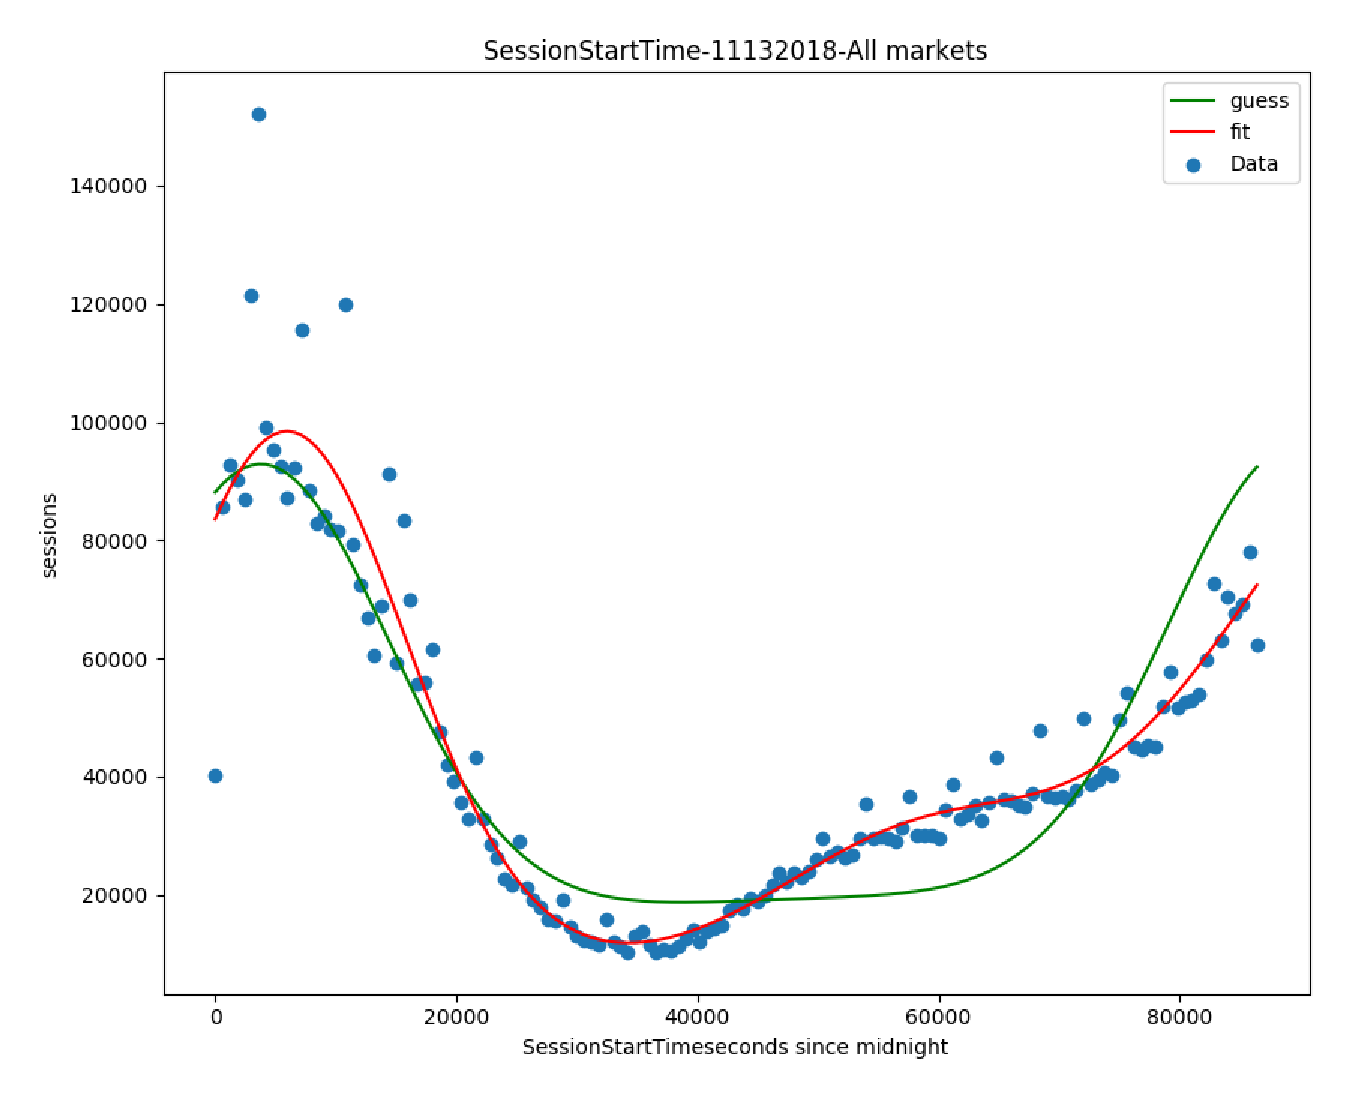
\includegraphics[width=\textwidth]
        {figures/fittedDailyUse.eps}}
        \caption{\label{FIGURE-DailyUse} An aggregated example one day usage from all markets. Ten minute bins. Fitted to smooth function.}
      \end{figure}

\begin{figure}[!htb]
        \center{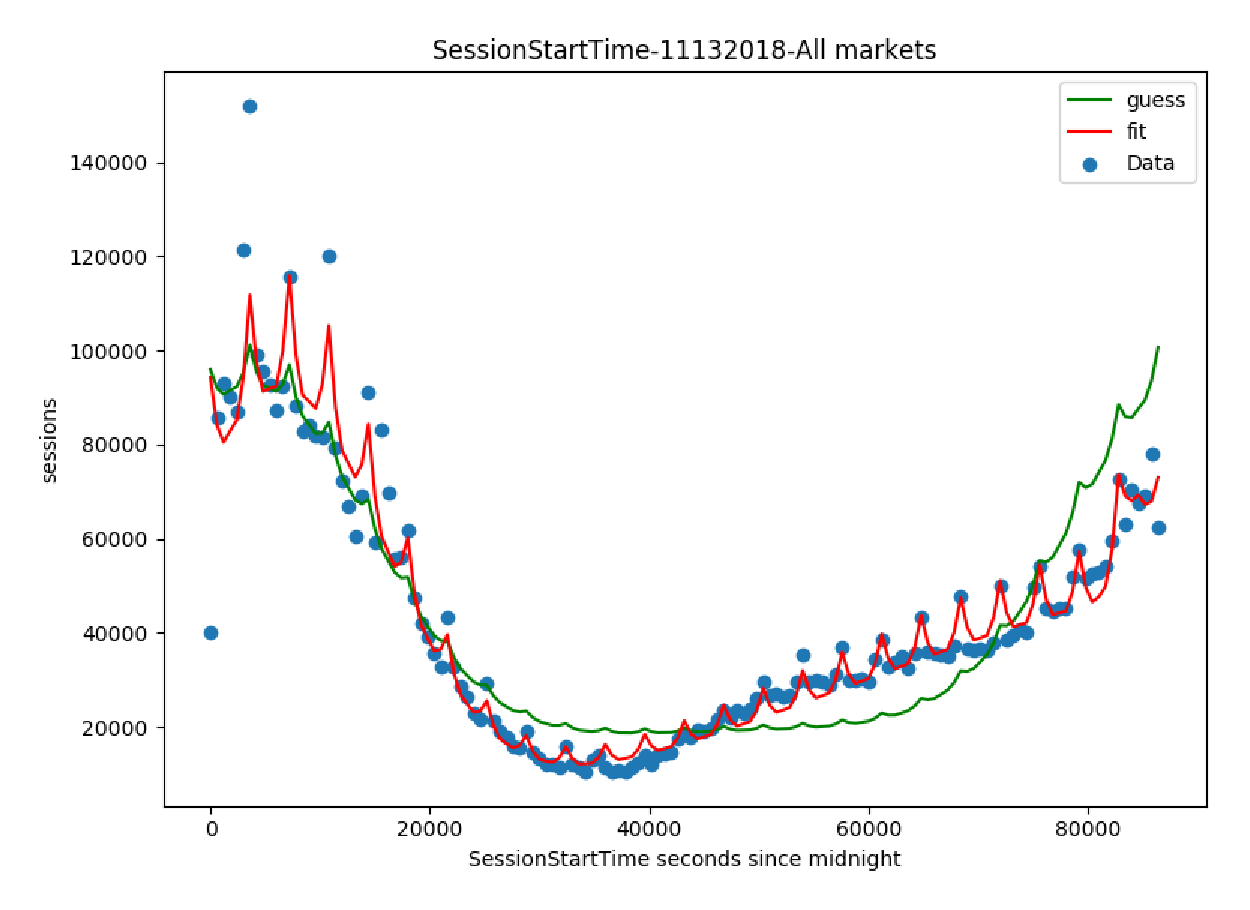
\includegraphics[width=\textwidth]
        {figures/fittedDailyUseWithSpikes.eps}}
        \caption{\label{FIGURE-DailyUseWithSpikes} An aggregated example one day usage from all markets. Ten minute bins. Fitted with peak usage.}
      \end{figure}

A distinction should be made between prime time load, and peak prime time load. A fit to the data will return prime time load which was used in this analysis as in figure~\ref{FIGURE-DailyUse}, but every 30 minutes on the half hour a spike in usage occurs. Those spikes (peak prime time load), example shown in figure~\ref{FIGURE-DailyUseWithSpikes} can be up to 2x the result from the fitted prime time load. If peak prime time analysis is preferred estimate double the stitcher need. Prime time concourrent sessions can be seen in table~\ref{TABLE-marketConcSessions}.

\begin{table}
\begin{tabular}{|l|l|} 
\hline Market & Prime Time Concourrent Sessions \\
\hline BHDCAL & 1,350 \\
\hline EDPRMN & 1,500 \\
\hline KNWDMI & 3,900 \\
\hline MDDCWI & 3,750 \\
\hline PLDCOR & 1,050 \\
\hline RENONV & 2,000 \\
\hline SLDCMO & 5,250 \\
\hline SPDCSC & 3,000 \\
\hline BODCMA & 1,050 \\
\hline DLDCTX & 1,500 \\
\hline LADCCA & 3,375 \\
\hline NVDCTN & 1,200 \\
\hline SLDCLA & 675 \\
\hline SLOTCA & 450 \\
\hline TWCCA & 3,750 \\
\hline TWCNY.NYDC & 1,500 \\
\hline TWCNY.SYDC & 3,000 \\
\hline TWCOH & 6,000 \\
\hline TWCSC & 6,000 \\
\hline TWCTX & 6,000 \\
\hline 
\end{tabular}
\caption{\label{TABLE-marketConcSessions}Estimated number of concourrent sessions by market}
\end{table}

Functional forms for the fits shown in figures~\ref{FIGURE-DailyUse}~and~\ref{FIGURE-DailyUseWithSpikes} are $$ \frac{1}{\sqrt{2*\pi}} * [ \frac{\alpha}{\sigma_1} * e^{\frac{-1*(x-\mu_1)^{2}}{2*\sigma_1^{2}}} + \frac{\beta}{\sigma_2} * e^{\frac{-1*(x-\mu_2)^{2}}{2*\sigma_2^{2}}} + \frac{\gamma}{\sigma_3} * e^{\frac{-1*(x-\mu_3)^{2}}{2*\sigma_3^{2}}}] + C$$ and  $$ \frac{1}{\sqrt{2*\pi}} * [ \frac{\alpha}{\sigma_1} * e^{\frac{-1*(x-\mu_1)^{2}}{2*\sigma_1^{2}}} + \frac{\beta}{\sigma_2} * e^{\frac{-1*(x-\mu_2)^{2}}{2*\sigma_2^{2}}} + \frac{\gamma}{\sigma_3} * e^{\frac{-1*(x-\mu_3)^{2}}{2*\sigma_3^{2}}}]* [1+A*cos(\pi*x/3600)^{8}] + C$$ where the fit parameters are $\alpha, \beta, \gamma, \mu_1, \mu_2, \mu_3, \sigma_1, \sigma_2, \sigma_3, A,$ and $C$. The base funcion is three gaussians, one for prime time, one ramping up into prime time of next day, and one for mid-day viewership. The enveloped $cos^{8}$ function is meant to account for increased viewership every 30 min between standard scheduled programs. This functional form can be made to fit any timeseries data observable in the spec guide ecosystem provided a reasonable guess to fit parameters can be provided and the feature has suficient statistics for fitting. 



\section{Stitcher Capacity Analysis}

Now that the pieces are in place we can begin calculation of stitcher capacity. There are three types of stitchers in production, those with 96 GB of memory, those with 128 GB, and those with 256 GB. The capacity of these stitchers is calculated by  $$Capacity=\frac{Mem * 0.8 * 1000}{SesSize + 2.32*SesVar}$$ Where $Capacity$ is the number of sessions a stitcher can take, $Mem$ is the memory of the stitcher in GB, $0.8$ is the threshold for avoiding stitcher degredation (alloting for some system proceses as well) $1000$ is a conversion factor, $SesSize$ is the average size of sessions in MB, $SesVar$ is the standard deviation of session size, and the $2.32$ factor is a Z-score corresponding to a 1\% chance of stitcher degredation. The results can be calculated market by market but in the end all markets are exhibiting similar behaviour and for the observed size of sessions capacity is summarized in table~\ref{TABLE-StitcherCapacity}.

\begin{table}
\begin{tabular}{|l|l|} 
\hline Stitcher Memory (GB) & Stitcher Capacity (sessions) \\
\hline 96 & 20 \\
\hline 128 & 65 \\
\hline 256 & 125 \\
\hline 
\end{tabular}
\caption{\label{TABLE-StitcherCapacity}Stitcher Capacity by type of stitcher}
\end{table}



\section{Stitchers Available}

Before we can calculate how much capacity our markets have, we need to know how many and of what kind of stitchers are available merket by market. A summary can be seen in table~\ref{TABLE-marketStitcherAvail}.

\begin{table}
\begin{tabular}{|l|l|l|} 
\hline Market & Number of stitchers available & Memory of stitchers on market \\
\hline BHDCAL & 111 & 96 \\
\hline EDPRMN & 89 & 96 \\
\hline KNWDMI & 149 & 96 \\
\hline MDDCWI & 187 & 96 \\
\hline PLDCOR & 50 & 96 \\
\hline RENONV & 56 & 96 \\
\hline SLDCMO & 258 & 96 \\
\hline SPDCSC & 84 & 96 \\
\hline BODCMA & 55 & 128 \\
\hline DLDCTX & 23 & 128 \\
\hline LADCCA & 47 & 128 \\
\hline NVDCTN & 50 & 128 \\
\hline SLDCLA & 23 & 128 \\
\hline SLOTCA & 13 & 128 \\
\hline TWCCA & 287 & 256 \\
\hline TWCNY.NYDC & 323 & 256 \\
\hline TWCNY.SYDC & 323 & 256 \\
\hline TWCOH & 443 & 256 \\
\hline TWCSC & 307 & 256 \\
\hline TWCTX & 282 & 256 \\
\hline 
\end{tabular}
\caption{\label{TABLE-marketStitcherAvail}Stitcher availability market by market.} 
\end{table}



\section{Market Capacity Analysis}

With the number of sessions that we need to support the current environment right now, and the number of sessions a stitcher can handle with acceptable error rates, the number of stitchers needed to support our customers can be calculated. We can also cacluate the need if we upgrade to 256 GB stitchers and project how many stitchers we need in order to achieve our growth expectations growing from 2 million customers to 8 million customers by end of year. Lacking growth models for use in this analysis it is assumed that all markets will grow equally maintaining their current market share. The results are summarized in table~\ref{TABLE-StitchersNeeded}. Take special note of cases where the number of stitchers needed right now exceeds availability (highlighted orange) and cases where we are very nearly at full capacity (highlighted yellow). 

\begin{table}
\begin{tabular}{|l|p{17mm}|p{17mm}|p{17mm}|p{17mm}|p{17mm}|p{17mm}|} 
\hline Market & N stitchers available & Memory of stitchers on market & N stitchers needed NOW & N 256GB stitchers needed now & N stitchers needed by eoy & N 256GB stitchers needed by eoy \\
\hline BHDCAL & 111 & 96 & 27 & 10 & 109 & 41 \\
\hline EDPRMN & 89 & 96 & 70 & 26 & 280 & 105 \\
\rowcolor{orange}\hline KNWDMI & 149 & 96 & 167 & 63 & 669 & 251 \\
\rowcolor{orange}\hline MDDCWI & 187 & 96 & 188 & 70 & 751 & 281 \\
\rowcolor{yellow}\hline PLDCOR & 50 & 96 & 49 & 18 & 196 & 74 \\
\rowcolor{orange}\hline RENONV & 56 & 96 & 80 & 30 & 321 & 120 \\
\hline SLDCMO & 258 & 96 & 219 & 82 & 876 & 328 \\
\rowcolor{orange}\hline SPDCSC & 84 & 96 & 141 & 53 & 565 & 212 \\
\hline BODCMA & 55 & 128 & 17 & 8 & 67 & 33 \\
\rowcolor{yellow}\hline DLDCTX & 23 & 128 & 23 & 11 & 92 & 46 \\
\rowcolor{yellow}\hline LADCCA & 47 & 128 & 46 & 23 & 182 & 91 \\
\hline NVDCTN & 50 & 128 & 21 & 11 & 86 & 43 \\
\hline SLDCLA & 23 & 128 & 13 & 7 & 52 & 26 \\
\hline SLOTCA & 13 & 128 & 6 & 3 & 26 & 13 \\
\hline TWCCA & 287 & 256 & 30 & 30 & 120 & 120 \\
\hline TWCNY.NYDC & 323 & 256 & 12 & 12 & 47 & 47 \\
\hline TWCNY.SYDC & 323 & 256 & 23 & 23 & 94 & 94 \\
\hline TWCOH & 443 & 256 & 46 & 46 & 185 & 185 \\
\hline TWCSC & 307 & 256 & 49 & 49 & 194 & 194 \\
\hline TWCTX & 282 & 256 & 46 & 46 & 184 & 184 \\
\hline 
\end{tabular}
\caption{\label{TABLE-StitchersNeeded}Stitcher availability market by market.} 
\end{table}



\newpage



\appendix
\section{Session Size Tables}
\label{SECTION-SessionTables}

\begin{tabular}{|l|l|l|l|l|}
\hline 
\hline All markets & ELAPSED &        CPU\% &      RSS(mb) &     SIZE(mb) \\
\hline count &                   7964 &  7964.000000 &  7964.000000 &   7964.00000 \\
\hline mean &   0 days 16:57:29.043571 &    6.670191 &   704.325508 &  1016.00872 \\
\hline std &    6 days 12:33:38.785822 &   17.375503 &   587.128283 &   751.04424 \\
\hline min &         0 days 00:00:00 &    0.000000 &    26.296000 &    37.20400 \\
\hline 25\% &           0 days 00:04:08 &    0.300000 &   306.063000 &   502.49400 \\
\hline 50\% &   0 days 00:28:41.500000 &    0.900000 &   604.702000 &   906.51000 \\
\hline 75\%  &         0 days 01:13:26 &    4.500000 &   888.213000 &  1256.41700 \\
\hline max &       131 days 03:35:10 &  145.000000 & 14712.656000 & 16320.25200 \\
\hline 
\end{tabular}


\begin{tabular}{|l|l|l|l|l|}
\hline 
\hline twctx& ELAPSED&  CPU\%&  RSS(mb)&  SIZE(mb) \\
\hline count&   1234& 1234.000000& 1234.000000& 1234.00000 \\
\hline mean&  0 days 00:38:16.789303&   4.593112&  490.834882&  751.81550 \\
\hline std&  0 days 00:58:26.775946&  10.083455&  253.906020&  352.73699 \\
\hline min&   0 days 00:00:00&   0.000000&  25.388000&  69.82800 \\
\hline 25\%&  0 days 00:03:03.750000&   0.300000&  272.858000&  446.80800 \\
\hline 50\%&   0 days 00:18:51&   0.900000&  366.556000&  588.50600 \\
\hline 75\%&  0 days 00:53:25.750000&   4.700000&  670.100000& 1007.64800 \\
\hline max&   0 days 14:24:02&  130.000000& 1614.120000& 2286.67600 \\
\hline 
\end{tabular}


\begin{tabular}{|l|l|l|l|l|}
\hline 
\hline spdcsc& ELAPSED&    CPU\%&   RSS(mb)&  SIZE(mb) \\
\hline count&   1344& 1344.000000&  1344.000000&  1344.00000 \\
\hline mean&  0 days 05:33:22.727678&  10.047545&  747.331970&  1148.42780 \\
\hline std&  1 days 02:24:33.678990&  22.922085&  744.264176&  1063.67384 \\
\hline min&   0 days 00:00:00&   0.000000&  108.732000&  163.03600 \\
\hline 25\%&  0 days 00:03:07.500000&   0.400000&  363.873000&  616.14000 \\
\hline 50\%&  0 days 00:21:37.500000&   1.300000&  617.814000&  876.55200 \\
\hline 75\%&  0 days 01:02:09.250000&   7.300000&  818.191000&  1253.15700 \\
\hline max&  10 days 03:05:09&  154.000000& 11340.324000& 12773.81600 \\
\hline 
\end{tabular}
 
\begin{tabular}{|l|l|l|l|l|}
\hline 
\hline mddcwi& ELAPSED&   CPU\%&  RSS(mb)&   SIZE(mb) \\
\hline count&    663& 663.000000&  663.000000&  663.00000 \\
\hline mean&  0 days 01:13:31.853695&  7.504827&  871.828561& 1323.55937 \\
\hline std&  0 days 05:18:41.994081&  17.288993&  697.919157& 1085.96406 \\
\hline min&   0 days 00:00:01&  0.000000&  155.052000&  222.77200 \\
\hline 25\%&   0 days 00:03:22&  0.400000&  311.396000&  528.56600 \\
\hline 50\%&   0 days 00:21:19&  1.300000&  710.036000& 1025.54400 \\
\hline 75\%&  0 days 00:57:54.500000&  6.350000& 1140.840000& 1598.61800 \\
\hline max&   3 days 03:49:19&  99.800000& 5271.756000& 8797.68000 \\
\hline 
\end{tabular}
 
\begin{tabular}{|l|l|l|l|l|}
\hline 
\hline bhnoh&    ELAPSED&   CPU\%&  RSS(mb)&   SIZE(mb) \\
\hline count&    38& 38.000000&  38.000000&  38.00000 \\
\hline mean&  45 days 04:09:45.289473& 92.215789&  578.135263&  953.34589 \\
\hline std&  41 days 20:07:34.367849& 26.600442&  98.453239&  173.38133 \\
\hline min&   0 days 00:07:49&  1.200000&  453.460000&  751.18400 \\
\hline 25\%&  28 days 09:15:25.250000& 99.900000&  542.662000&  894.69800 \\
\hline 50\%&   28 days 17:57:53& 99.900000&  556.336000&  918.71400 \\
\hline 75\%&  29 days 04:38:27.750000& 99.900000&  582.774000&  981.54900 \\
\hline max&  130 days 15:53:57& 99.900000& 1052.028000& 1736.06000 \\
\hline 
\end{tabular}
 
\begin{tabular}{|l|l|l|l|l|}
\hline 
\hline twcsc& ELAPSED&   CPU\%&  RSS(mb)&   SIZE(mb) \\
\hline count&    697& 697.000000&  697.000000&  697.00000 \\
\hline mean&  0 days 02:14:16.459110&  5.776327&  497.244746&  757.31775 \\
\hline std&  0 days 21:17:15.405321&  13.323263&  287.396410&  387.90609 \\
\hline min&   0 days 00:00:00&  0.000000&  36.252000&  82.15600 \\
\hline 25\%&   0 days 00:02:47&  0.300000&  273.080000&  447.08000 \\
\hline 50\%&   0 days 00:17:00&  1.000000&  347.376000&  561.42400 \\
\hline 75\%&   0 days 00:53:12&  5.500000&  693.360000& 1035.06000 \\
\hline max&  14 days 02:01:05& 101.000000& 2512.328000& 3058.43600 \\
\hline 
\end{tabular}
 
\begin{tabular}{|l|l|l|l|l|}
\hline 
\hline slotca&    ELAPSED&   CPU\%&  RSS(mb)&   SIZE(mb) \\
\hline count&   189& 189.000000&  189.000000&  189.00000 \\
\hline mean&  2 days 05:08:17.068783&  10.966667&  517.918413&  743.12943 \\
\hline std&  12 days 06:00:47.279801&  23.232777&  254.689270&  314.38865 \\
\hline min&   0 days 00:00:00&  0.000000&  68.068000&  113.12400 \\
\hline 25\%&   0 days 00:02:09&  0.400000&  291.140000&  466.89600 \\
\hline 50\%&   0 days 00:13:11&  1.900000&  506.636000&  705.66000 \\
\hline 75\%&   0 days 00:58:16&  8.800000&  690.876000&  947.54800 \\
\hline max&  103 days 06:27:34& 100.000000& 1366.460000& 1732.20800 \\
\hline 
\end{tabular}
 
\begin{tabular}{|l|l|l|l|l|}
\hline 
\hline ladcca& ELAPSED&   CPU\%&  RSS(mb)&   SIZE(mb) \\
\hline count&    867& 867.000000&  867.000000&  867.00000 \\
\hline mean&  0 days 08:47:35.552479&  8.360208&  450.936166&  669.28376 \\
\hline std&  2 days 16:09:18.559904&  18.904368&  244.823500&  307.58961 \\
\hline min&   0 days 00:00:00&  0.000000&  12.792000&  22.89200 \\
\hline 25\%&  0 days 00:01:21.500000&  0.400000&  275.056000&  466.51000 \\
\hline 50\%&   0 days 00:09:43&  1.400000&  336.452000&  557.32000 \\
\hline 75\%&  0 days 00:47:16.500000&  7.850000&  594.040000&  820.15200 \\
\hline max&  28 days 05:24:52& 150.000000& 1996.924000& 2973.56800 \\
\hline 
\end{tabular}
 
\begin{tabular}{|l|l|l|l|l|}
\hline 
\hline bhnfl&    ELAPSED&   CPU\%&   RSS(mb)&   SIZE(mb) \\
\hline count&    12&  12.000000&  12.000000&  12.00000 \\
\hline mean&   97 days 22:32:49&  76.050000& 488.248333&  816.10533 \\
\hline std&   59 days 00:42:48.484789&  43.274063& 128.220732&  184.42619 \\
\hline min&    0 days 00:02:23&  0.200000& 219.072000&  375.20800 \\
\hline 25\%&   97 days 20:51:46.250000&  76.625000& 451.802000&  774.66400 \\
\hline 50\%&   130 days 12:32:55&  99.900000& 489.430000&  791.46800 \\
\hline 75\%&  130 days 14:56:07.750000& 100.000000& 501.310000&  862.90800 \\
\hline max&   130 days 16:14:00& 100.000000& 797.216000& 1138.86400 \\
\hline 
\end{tabular}
 
\begin{tabular}{|l|l|l|l|l|}
\hline 
\hline twcoh& ELAPSED&   CPU\%&  RSS(mb)&   SIZE(mb) \\
\hline count&    611& 611.000000&  611.000000&  611.00000 \\
\hline mean&  0 days 00:41:26.962356&  4.990344&  499.298710&  762.94798 \\
\hline std&  0 days 00:55:17.385177&  10.710850&  253.252774&  350.21950 \\
\hline min&   0 days 00:00:00&  0.000000&  18.548000&  55.67600 \\
\hline 25\%&  0 days 00:03:01.500000&  0.300000&  282.944000&  460.38400 \\
\hline 50\%&   0 days 00:20:57&  0.800000&  373.420000&  609.91200 \\
\hline 75\%&   0 days 00:59:45&  4.300000&  683.328000& 1013.02800 \\
\hline max&   0 days 07:08:58&  90.500000& 1385.548000& 2101.02800 \\
\hline 
\end{tabular}
 
\begin{tabular}{|l|l|l|l|l|}
\hline 
\hline sldcmo& ELAPSED&   CPU\%&  RSS(mb)&   SIZE(mb) \\
\hline count&    811& 811.000000&  811.000000&  811.00000 \\
\hline mean&  0 days 00:48:12.890258&  4.603083&  991.308099& 1350.01964 \\
\hline std&  0 days 01:16:55.655732&  9.059367&  681.528005&  798.25732 \\
\hline min&   0 days 00:00:00&  0.000000&  140.636000&  225.09600 \\
\hline 25\%&   0 days 00:04:00&  0.400000&  402.364000&  658.48400 \\
\hline 50\%&   0 days 00:24:37&  1.200000&  858.612000& 1207.46800 \\
\hline 75\%&  0 days 00:58:13.500000&  4.700000& 1315.152000& 1718.66600 \\
\hline max&   0 days 16:32:18&  93.000000& 4124.472000& 5313.78000 \\
\hline 
\end{tabular}
 
\begin{tabular}{|l|l|l|l|l|}
\hline 
\hline knwdmi& ELAPSED&   CPU\%&   RSS(mb)&  SIZE(mb) \\
\hline count&    854& 854.000000&  854.000000&  854.00000 \\
\hline mean&  0 days 01:50:32.909836&  7.179040&  742.129691&  1106.20582 \\
\hline std&  0 days 11:45:10.901628&  16.393025&  730.700326&  942.02897 \\
\hline min&   0 days 00:00:01&  0.000000&  124.752000&  209.78000 \\
\hline 25\%&   0 days 00:02:39&  0.400000&  371.277000&  626.71100 \\
\hline 50\%&  0 days 00:18:28.500000&  1.100000&  638.800000&  933.37400 \\
\hline 75\%&   0 days 00:51:55&  6.575000&  920.667000&  1273.83700 \\
\hline max&   7 days 07:38:22& 111.000000& 13115.864000& 14916.46000 \\
\hline 
\end{tabular}
 
\begin{tabular}{|l|l|l|l|l|}
\hline 
\hline bhnca&    ELAPSED& CPU\%& RSS(mb)& SIZE(mb) \\
\hline count&    1&  1.0&   1.00&  1.0 \\
\hline mean&  0 days 00:00:06& 30.5&  247.74&  404.7 \\
\hline std&    NaT&  NaN&  NaN&   NaN \\
\hline min&  0 days 00:00:06& 30.5&  247.74&  404.7 \\
\hline 25\%&  0 days 00:00:06& 30.5&  247.74&  404.7 \\
\hline 50\%&  0 days 00:00:06& 30.5&  247.74&  404.7 \\
\hline 75\%&  0 days 00:00:06& 30.5&  247.74&  404.7 \\
\hline max&  0 days 00:00:06& 30.5&  247.74&  404.7 \\
\hline 
\end{tabular}
 
\begin{tabular}{|l|l|l|l|l|}
\hline 
\hline twcny.sydc& ELAPSED&   CPU\%&  RSS(mb)&   SIZE(mb) \\
\hline count&    442& 442.000000&  442.000000&  442.00000 \\
\hline mean&  0 days 01:01:03.726244&  6.148190&  500.684950&  763.87129 \\
\hline std&  0 days 05:46:28.356034&  15.162467&  260.041742&  358.83244 \\
\hline min&   0 days 00:00:00&  0.000000&  84.572000&  132.11200 \\
\hline 25\%&   0 days 00:03:06&  0.300000&  276.576000&  455.65000 \\
\hline 50\%&   0 days 00:22:50&  0.800000&  367.764000&  581.14200 \\
\hline 75\%&  0 days 00:59:00.750000&  4.875000&  697.221000& 1039.71500 \\
\hline max&   3 days 13:49:05& 118.000000& 1466.484000& 1944.98800 \\
\hline 
\end{tabular}
 
\begin{tabular}{|l|l|l|l|l|}
\hline 
\hline sldcla& ELAPSED&   CPU\%&  RSS(mb)&   SIZE(mb) \\
\hline count&    358& 358.000000&  358.000000&  358.00000 \\
\hline mean&  0 days 00:58:12.290502&  6.725419&  680.787911&  928.31454 \\
\hline std&  0 days 05:02:56.766229&  14.714847&  384.019453&  454.63616 \\
\hline min&   0 days 00:00:00&  0.000000&  24.804000&  55.67600 \\
\hline 25\%&   0 days 00:01:33&  0.300000&  314.110000&  508.44400 \\
\hline 50\%&   0 days 00:16:41&  1.300000&  614.728000&  848.91000 \\
\hline 75\%&  0 days 00:54:09.250000&  6.300000&  965.019000& 1233.39500 \\
\hline max&   3 days 22:07:52& 105.000000& 1957.948000& 2583.84800 \\
\hline 
\end{tabular}
 
\begin{tabular}{|l|l|l|l|l|}
\hline 
\hline edprmn&    ELAPSED&   CPU\%&   RSS(mb)&  SIZE(mb) \\
\hline count&   703& 703.000000&  703.000000&  703.00000 \\
\hline mean&  3 days 23:41:03.660028&  9.510953&  687.757826&  1037.11116 \\
\hline std&  14 days 10:19:40.838831&  19.807971&  875.313315&  1095.16143 \\
\hline min&   0 days 00:00:00&  0.000000&   26.296000&   37.20400 \\
\hline 25\%&   0 days 00:01:28&  0.400000&  299.240000&  519.00800 \\
\hline 50\%&   0 days 00:13:56&  1.700000&  563.340000&  828.87200 \\
\hline 75\%&   0 days 00:52:57&  9.950000&  807.120000&  1152.59800 \\
\hline max&   61 days 20:24:45& 136.000000& 12119.260000& 13713.00400 \\
\hline 
\end{tabular}
 
\begin{tabular}{|l|l|l|l|l|}
\hline 
\hline bhnal&    ELAPSED&   CPU\%&   RSS(mb)&  SIZE(mb) \\
\hline count&   703& 703.000000&  703.000000&  703.00000 \\
\hline mean&  3 days 23:41:03.660028&  9.510953&  687.757826&  1037.11116 \\
\hline std&  14 days 10:19:40.838831&  19.807971&  875.313315&  1095.16143 \\
\hline min&   0 days 00:00:00&  0.000000&   26.296000&   37.20400 \\
\hline 25\%&   0 days 00:01:28&  0.400000&  299.240000&  519.00800 \\
\hline 50\%&   0 days 00:13:56&  1.700000&  563.340000&  828.87200 \\
\hline 75\%&   0 days 00:52:57&  9.950000&  807.120000&  1152.59800 \\
\hline max&   61 days 20:24:45& 136.000000& 12119.260000& 13713.00400 \\
\hline 
\end{tabular}
 
\begin{tabular}{|l|l|l|l|l|}
\hline 
\hline twcny.nydc& ELAPSED&   CPU\%&  RSS(mb)&   SIZE(mb) \\
\hline count&    439& 439.000000&  439.000000&  439.00000 \\
\hline mean&  0 days 00:42:33.881548&  3.782232&  505.566378&  770.06229 \\
\hline std&  0 days 00:56:37.780297&  10.605681&  253.195549&  353.68918 \\
\hline min&   0 days 00:00:00&  0.000000&  84.100000&  132.11200 \\
\hline 25\%&  0 days 00:05:23.500000&  0.200000&  284.092000&  456.28800 \\
\hline 50\%&   0 days 00:25:12&  0.700000&  413.500000&  646.48800 \\
\hline 75\%&  0 days 00:54:22.500000&  2.350000&  682.940000& 1027.04000 \\
\hline max&   0 days 07:27:59& 119.000000& 1451.068000& 1988.59200 \\
\hline 
\end{tabular}
 
\begin{tabular}{|l|l|l|l|l|}
\hline 
\hline renonv& ELAPSED&   CPU\%&  RSS(mb)&   SIZE(mb) \\
\hline count&    990& 990.000000&  990.000000&  990.00000 \\
\hline mean&  0 days 01:00:09.429292&  4.826869&  968.266428& 1315.58436 \\
\hline std&  0 days 01:28:07.999288&  11.318484&  643.358079&  761.49195 \\
\hline min&   0 days 00:00:00&  0.000000&  87.840000&  156.11200 \\
\hline 25\%&  0 days 00:04:56.250000&  0.400000&  407.672000&  640.68700 \\
\hline 50\%&  0 days 00:32:28.500000&  0.900000&  857.420000& 1223.10600 \\
\hline 75\%&  0 days 01:13:59.750000&  4.000000& 1267.769000& 1644.98900 \\
\hline max&   0 days 17:49:29& 100.000000& 4509.704000& 5523.24800 \\
\hline 
\end{tabular}
 
\begin{tabular}{|l|l|l|l|l|}
\hline 
\hline dldctx& ELAPSED&    CPU\%&  RSS(mb)&   SIZE(mb) \\
\hline count&   1240& 1240.000000& 1240.000000& 1240.00000 \\
\hline mean&  0 days 09:59:56.741129&   9.365484&  484.178539&  729.23009 \\
\hline std&  3 days 22:37:16.728882&  18.061337&  295.350663&  359.44808 \\
\hline min&   0 days 00:00:00&   0.000000&  84.692000&  132.11200 \\
\hline 25\%&   0 days 00:01:12&   0.600000&  274.080000&  477.95400 \\
\hline 50\%&  0 days 00:04:50.500000&   3.300000&  343.756000&  568.51400 \\
\hline 75\%&   0 days 00:38:54&   9.250000&  635.297000&  909.19700 \\
\hline max&  70 days 04:14:55&  119.000000& 2011.240000& 2581.69200 \\
\hline 
\end{tabular}
 
\begin{tabular}{|l|l|l|l|l|}
\hline 
\hline bhdcal&    ELAPSED&   CPU\%&  RSS(mb)&   SIZE(mb) \\
\hline count&   449& 449.000000&  449.000000&  449.00000 \\
\hline mean&  3 days 10:05:22.552338&  12.213586&  511.082013&  745.66570 \\
\hline std&  15 days 10:04:40.019196&  27.009075&  278.026679&  344.30193 \\
\hline min&   0 days 00:00:00&  0.000000&  107.364000&  158.71200 \\
\hline 25\%&   0 days 00:03:04&  0.500000&  296.092000&  492.30400 \\
\hline 50\%&   0 days 00:22:34&  1.400000&  424.240000&  654.30800 \\
\hline 75\%&   0 days 01:02:13&  7.300000&  660.296000&  913.29200 \\
\hline max&  116 days 16:49:08& 115.000000& 1892.232000& 2884.86400 \\
\hline 
\end{tabular}
 
\begin{tabular}{|l|l|l|l|l|}
\hline 
\hline twchi& ELAPSED& CPU\%& RSS(mb)& SIZE(mb) \\
\hline count&    0&   0&   0& 0    \\
\hline unique&   0&   0&   0& 0    \\
\hline 
\end{tabular}
 
\begin{tabular}{|l|l|l|l|l|}
\hline 
\hline pldcor& ELAPSED&   CPU\%&  RSS(mb)&   SIZE(mb) \\
\hline count&    389& 389.000000&  389.000000&  389.00000 \\
\hline mean&  1 days 05:24:52.033419&  11.805141&  815.620380& 1175.33370 \\
\hline std&  5 days 16:38:37.442890&  24.115209&  733.513476& 1041.47454 \\
\hline min&   0 days 00:00:01&  0.000000&  125.612000&  211.30800 \\
\hline 25\%&   0 days 00:01:08&  0.300000&  330.576000&  576.40000 \\
\hline 50\%&   0 days 00:14:33&  2.300000&  636.780000&  919.36800 \\
\hline 75\%&   0 days 01:38:37&  8.500000& 1054.984000& 1405.63200 \\
\hline max&  37 days 14:45:31&  99.900000& 6727.340000& 8748.13200 \\
\hline 
\end{tabular}
 
\begin{tabular}{|l|l|l|l|l|}
\hline 
\hline bodcma& ELAPSED&   CPU\%&  RSS(mb)&   SIZE(mb) \\
\hline count&    593& 593.000000&  593.000000&  593.00000 \\
\hline mean&  0 days 00:33:41.399662&  5.413322&  537.107386&  765.38517 \\
\hline std&  0 days 00:44:57.083644&  12.469223&  307.470807&  369.60064 \\
\hline min&   0 days 00:00:00&  0.000000&  144.824000&  210.89600 \\
\hline 25\%&   0 days 00:01:55&  0.300000&  280.832000&  462.84000 \\
\hline 50\%&   0 days 00:17:30&  1.000000&  412.584000&  637.72800 \\
\hline 75\%&   0 days 00:49:06&  5.200000&  722.672000&  989.54400 \\
\hline max&   0 days 08:33:57& 153.000000& 2237.936000& 2545.99200 \\
\hline 
\end{tabular}
 
\begin{tabular}{|l|l|l|l|l|}
\hline 
\hline twcca& ELAPSED&   CPU\%&  RSS(mb)&   SIZE(mb) \\
\hline count&    505& 505.000000&  505.000000&  505.00000 \\
\hline mean&  0 days 00:35:02.885148&  4.480000&  515.805513&  793.22996 \\
\hline std&  0 days 00:45:24.634973&  8.867115&  255.678862&  365.21607 \\
\hline min&   0 days 00:00:00&  0.000000&  122.608000&  176.76000 \\
\hline 25\%&   0 days 00:03:25&  0.300000&  288.092000&  459.67200 \\
\hline 50\%&   0 days 00:18:04&  0.900000&  398.276000&  666.70800 \\
\hline 75\%&   0 days 00:50:38&  4.200000&  702.064000& 1059.37600 \\
\hline max&   0 days 05:29:07&  82.500000& 1365.628000& 1919.64400 \\
\hline 
\end{tabular}
 
\begin{tabular}{|l|l|l|l|l|}
\hline 
\hline nvdctn&    ELAPSED&   CPU\%&  RSS(mb)&   SIZE(mb) \\
\hline count&   773& 773.000000&  773.000000&  773.00000 \\
\hline mean&  1 days 23:34:24.972833&  9.574774&  581.608310&  834.08841 \\
\hline std&  11 days 21:42:02.836950&  21.275061&  351.990133&  428.15494 \\
\hline min&   0 days 00:00:00&  0.000000&  55.104000&  105.19200 \\
\hline 25\%&   0 days 00:02:02&  0.400000&  299.696000&  492.51200 \\
\hline 50\%&   0 days 00:19:12&  1.500000&  499.720000&  732.01600 \\
\hline 75\%&   0 days 00:56:50&  7.900000&  779.652000& 1067.57600 \\
\hline max&  127 days 05:50:07& 115.000000& 2500.564000& 3165.04800 \\
\hline 
\end{tabular}
 
\begin{tabular}{|l|l|l|l|l|}
\hline 
\hline blngmt& ELAPSED&   CPU\%&  RSS(mb)&   SIZE(mb) \\
\hline count&    269& 269.000000&  269.000000&  269.00000 \\
\hline mean&  0 days 00:37:08.981412&  5.629368&  547.594528&  775.47467 \\
\hline std&  0 days 00:54:32.902980&  9.371941&  439.892380&  541.74936 \\
\hline min&   0 days 00:00:00&  0.000000&  122.984000&  177.21200 \\
\hline 25\%&   0 days 00:01:03&  0.400000&  275.140000&  429.76800 \\
\hline 50\%&   0 days 00:14:04&  1.300000&  330.268000&  515.21600 \\
\hline 75\%&   0 days 00:54:23&  7.800000&  646.032000&  951.88400 \\
\hline max&   0 days 05:50:57&  67.500000& 2521.860000& 3125.04800 \\
\hline 
\end{tabular}



\end{document}
